\setcounter{chapter}{2}
\chapter{PRÉPARATION AU LANCEMENT}
\minitoc %insert la minitoc
\graphicspath{{Chapitre3/figures/}}

%\DoPToC

%==============================================================================
\pagestyle{fancy}
\fancyhf{}
\fancyhead[R]{\bfseries\rightmark}
\fancyfoot[R]{\thepage}
\renewcommand{\headrulewidth}{0.5pt}
\renewcommand{\footrulewidth}{0pt}
\renewcommand{\chaptermark}[1]{\markboth{\MakeUppercase{\chaptername~\thechapter. #1 }}{}}
\renewcommand{\sectionmark}[1]{\markright{\thechapter.\thesection~ #1}}

\begin{spacing}{1.5}

%==============================================================================
\section*{Introduction}
Avant d'appréhender le développment du système, il est primordial d'acquérir une compréhension claire des besoins des parties prenantes au projet, et des fonctionalités escomptées du système.\\
Ce chapitre couronne l'étape d'élaboration de la vision de notre produit, par la spécification des besoins. La phase d'inception se poursuit avec l'édification de l'architecture globale du produit et le choix de l'environnement technique. Ces deux parties conclueront le chapitre et annoncent l'achèvement de la phase d'inception.

%==============================================================================
\section{Analyse des besoins}
L'analyse des besoins a pour objectif l'identification des acteurs du système et de leurs rôles, ainsi que la spécification des besoins et des contraintes contre lesquelles le produit final sera validé. Il existe deux types de besoins :
\begin{itemize}
    \item Les besoisn fonctionnels, qui présentent ce que l'utilisateur attend en terme de service
    \item Les besoins non fonctionnels, qui présentent les contraintes sous lesquelles l'application doit être opérationnelle
\end{itemize}

%-----------------------------------------------------------------------------------
\subsection{Objet global du projet}
L'objectif du projet consiste à la conception, au développement, ainsi qu’au déploiement, d’une application web de gestion de projets, compatible avec tous les terminaux, de format réduit ou large, et disponible d’usage principalement en mode SaaS.\\
Pour toute organisation cliente, l’application permettra essentiellement aux responsables, chefs de projet, de gérer les différents aspects des projets entrepris par leur organisation, ainsi que d’en monitorer l’état.\\

Le produit final comportera ainsi deux parties distinctes :
\begin{itemize}
\item Une application web de gestion de projets en mode SaaS, ou à déploiement en interne
    \item Une solution complémentaire pour la gestion de l’aspect SaaS
\end{itemize}

%-----------------------------------------------------------------------------------
\subsection{Identification des acteurs}
L’application est destinée à être acquise par une organisation de petite ou de grande envergure (entreprise, équipe, …). Au sein de celle-ci, nous pouvons distinguer entre trois types d'acteurs à rôles distincts pour notre système :
\begin{itemize}
    \item \textbf{L'administrateur} : C’est l'utilisateur associé au compte existant par défaut lors de l'acquisition de la solution. Il possède les pleins pouvoirs sur le reste des comptes et a la charge de créer le autres comptes au tout début de la mise en route de l'application.
    \item \textbf{Un chef de projet} : C’est l'utilisateur fondamental du système. Il s'intéresse essentiellement à l'aspect de gestion de projets mais garde la possibilité de créer des comptes utilisateurs, à plus faible ou égal pouvoir, et de les gérer à sa guise.
    \item \textbf{Un intervenant} : Cet utilisateur est généralement externe à l'organisation et a pour but de contribuer à la gestion d'un projet. Son compte est créé par un chef de projet, ou l'administrateur, lequel lui procure des droits d'accès à différentes parties d'un projet, son rôle se restraignant à intervenir sur ces parties.
    \item \textbf{Un dirigeant} : Cet utilisateur, généralement interne à l'entreprise, s'intéresse et se limite uniquement à l'exploitation des fonctionalités de reporting offertes par le système, pour l'ensemble du portefeuille de projets. Son compte est créé et géré par l'administrateur.
    \item \textbf{Une partie prenante} : Cet utilisateur se limite à l'exploitation des fonctionalités de reporting offertes par le système dans le cadre d'un projet. Son compte est créé et géré par un chef de projet.
\end{itemize}
\

Pour la solution complémentaire de gestion de l’offre SaaS, on reconnait un type seul acteur, à savoir : L'administrateur SaaS. C’est lui qui gère les clients de l’offre SaaS. Il a la charge de monitorer l’usage de l’application en mode SaaS et de remédier aux requêtes des clients.

%-----------------------------------------------------------------------------------
\subsection{Spécification fonctionnelles}
On énumère ici les différentes contraintes et besoins fonctionnels requis de la part du livrable final.\\
L’application doit être en mesure d’offrir les fonctionnalités suivantes :
\begin{itemize}
    \item \textbf{Gestion du portefeuille de projets} : L'ensemble des projets du client doit être regoupé sous un portefeuille, qui offre des fonctionalités d'ajout et d'édition d'un ou plusieurs projets.
    \item \textbf{Gestion de la charte d'un projet} : Il s'agit d'offrir à l'utilisateur la possibilité de fournir les détails relatifs à la charte d'un projet dès sa création, tout en gardant la possibilité d'en éditer le contenu à postériori.
    \item \textbf{Reporting au niveau projet} : Une vue d'ensemble de l'état global d'un projet doit être accessible au travers d'un tableau de bord, contenant un agencement d'indicateurs clés pour le pilotage d'un projet.
    \item \textbf{Gestion de l'intégration} : Un projet doit pouvoir être structuré sous les différents niveaux suivants : projet, sous projet et chantier. Un projet peut inclure un ensemble de sous projets ou de chantiers, directemnt ratachés à lui. Un sous projet existe uniquement sous un projet, et peut lui-même contenir une multitude de chantiers, lui étant directement associés.
    \item \textbf{Gestion du plan d'action} : Une action est une tâche à réaliser, disposant essentiellement d'une description, d'un responsable et d'une date de clôture planifiée. Une action doit pouvoir être rajoutée sous n'importe quel niveau d'un projet, et peut être mise à jour ou bien supprimée. Un indicateur sur les actions en retard sera mis à disposition.
    \item \textbf{Gestion des coûts} : Le budget d'un projet ou d'un sous projet peut être renseigné et mis à jour tout au long de son existance. La gestion du budget inclut la spécification du budget initial, du buget consommé ainsi que d'une estimation du budget qui reste à consommer. Elle offre par ailleurs un indicateur sur le budget total prévisonnel.
    \item \textbf{Gestion du reste à faire} : Un reste à faire se distingue par une description et une charge associée, en homme / jour. Les restes à faire peuvent être créés et mis à jour, et sont rattachables à n'importe quel niveau d'un projet.
    \item \textbf{Planification} : La planification d'un projet ou d'un sous projet sera possible au travers de la création et de la consultation ultérieure des principaux jalons du niveau de projet. En essence, un jalon est défini par une brève description associée à une date d'échéance.
    \item \textbf{Gestion du "Scope"} : La gestion du "scope" ou du périmètre d'un niveau de projet s'accomplit principalement via la fourniture de documents en pièces jointes au niveau en question. D'autre part, la gestion du périmètre couvre la gestion du changement et des points en suspens. Un point en suspens est un point relatif au niveau de projet, en attente de résolution, auquel un responsable est assigné. La gestion du changement quant à elle est formalisée au travers de la soumission de demandes de changement. Chaque demande inclut essentiellement le demandeur ainsi que la décision prise par rapport à celle-ci.
    \item \textbf{Gestion des risques} : Le définition des risques peut être réalisée à n'importe quel niveau d'un projet. Un risque est défini par une description du risque encouru, associée à une probabilité et un impact. Ces derniers sont utilisés pour générer un indicateur sur le niveau de criticité (KRI \ref{ANGRAMME}) du risque. Leur suivi est réalisé principalement au travers de la spécification du statut, du plan d'action et des dispositions à prendre pour chaque risque, ainsi que d'une date de qualification et une date de clôture.
    \item \textbf{Gestion des ressources humaines} : La définition des ressources humaines peut être réalisée au niveau du portefeuille global de projets ou bien au niveau d'un projet ou d'un sous projet. Les ressources globales peuvent plus tard être assignées à un projet en particulier. Au sein d'un projet ou d'un sous projet, les ressources humaines peuvent être renseignées, mises à jour, et éventuellement assignées à une action ou un point en suspens. Une ressource humaine peut également être assignée en tant que responsable d'un plan de communication au niveau d'un projet.
    \item \textbf{Gestion de la communication} : La gestion de la communication se déroule au sein d'un projet. Elle inclut la définition de plans de communication, se distinguant par une description et un responsable communication, de même que la planification de réunions, disposant chacune d'un nom, d'une date et d'un lieu, acoompagnés d'un statut, ainsi que des comptes rendus de réunions.
    \item \textbf{Gestion des ressources non humaines} : Toute ressource matérielle ou immatérielle associée à un niveau de projet doit pouvoir être renseignée et mise à jour.
    \item \textbf{Publication de mises à jour} : L'état d'un projet doit pouvoir être archivé sous forme d'une mise à jour.
\end{itemize}
\

D'autre part, la solution adjointe de gestion du service SaaS devra quant à elle permettre de gérer les clients de l'offre SaaS : création d’un client, mise à jour des détails associées à un client et gestion du compte administrateur attaché.

%-----------------------------------------------------------------------------------
\subsection{Spécification non fonctionnelles}
En plus d’apporter les fonctionnalités citées précédemment, le produit final devra être en mesure d'assurer les aspects suivants :
\begin{itemize}
    \item \textbf{Sécurité} :
        \begin{itemize}
            \item[•] Isoler proprement les données des clients, et limiter efficacement leurs accès d'un client à un autre.
            \item[•] Mettre en place un système d’authentification et d’autorisation robuste.
        \end{itemize}
    \item \textbf{Performance} : Être réactive et relativement rapide lors de l'exécution.
    \item \textbf{Ergonomie} : Offrir une interface conviviale, intuitive et facile d’usage pour tous les types de dispositifs supportés.
    \item \textbf{Fiabilité} :
        \begin{itemize}
            \item[•] Conserver un comportement cohérent tout au long de la durée d'utilisation.
            \item[•] Éviter toute perte de donnée non intentionnelle.
            \item[•] Éviter ou résoudre les conflits engendrés par l’utilisation concurrente.
        \end{itemize}
    \item \textbf{Compatibilité} : Supporter la majorité des dispositifs des utilisateurs (smartphones, tablettes, ordinateurs, …) de manière adaptée à chacun.
    \item \textbf{Journalisation} :
        \begin{itemize}
            \item[•] Logging des événement importants.
            \item[•] Historiser l'état d'un projet et de ses mises à jour.
        \end{itemize}
\end{itemize}

%-----------------------------------------------------------------------------------
\subsection{Diagramme de cas d'utilisations}
La figure \ref{fig:useCasesDiag} illustre le diagramme de cas d'utilisation global de l'application. Il offre une représentation globale des principaux services offerts par le système, en fonction du type d'utilisateur.

\begin{figure}[H]
\centering
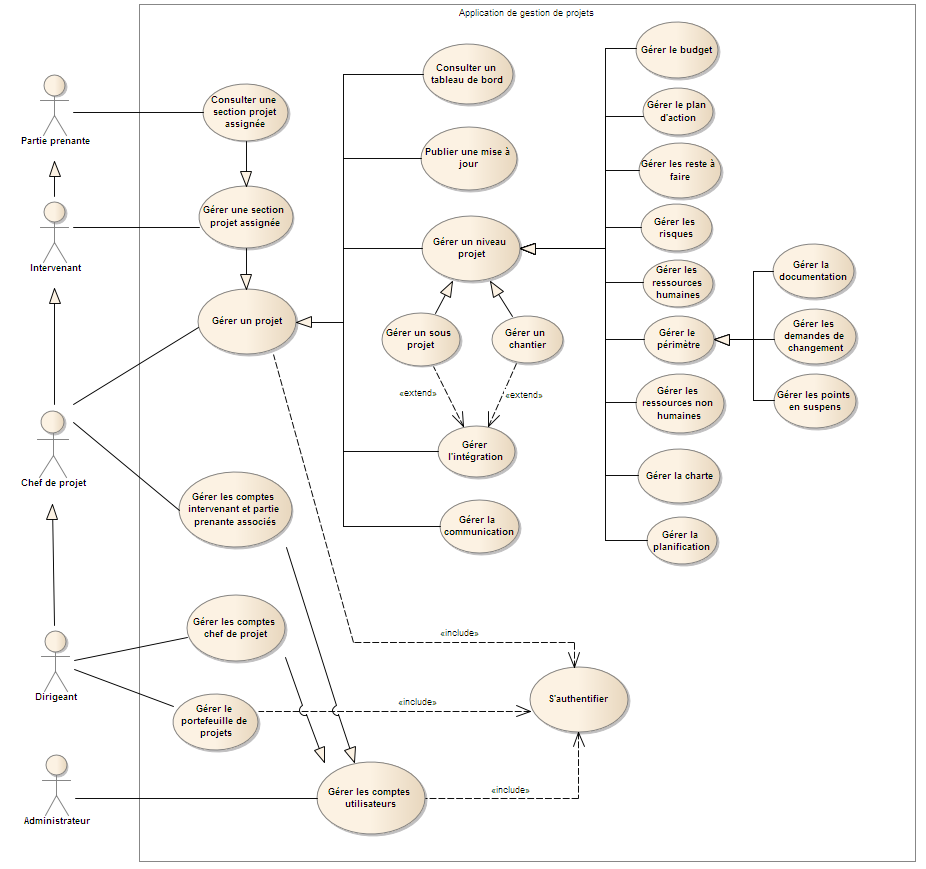
\includegraphics[width=1\linewidth]{useCasesDiag.png}
\caption{Diagramme global de cas d'utilisation}
\label{fig:useCasesDiag}
\end{figure}


%==============================================================================
\section{Étude technique}
Avant d'entamer la phase de développement, il est nécessaire de prendre du recul par rapport aux exigences et d'établir une vue d'ensemble du système d'un point de vue architectural. Dans notre cas en particulier, l'aspect SaaS de l'application impose une étude approfondie de l'infrastructure sous-jacente à mettre en place et des technologies à employer.

%-----------------------------------------------------------------------------------
\subsection{Architecture générale}
Une vue d'ensemble de l'architecture permet de mettre en évidence les différentes couches du système à développer.\\
Au vu du caractère Web de l'application, nous nous sommes d'abord orientés vers une architecture traditionnelle en 3-tiers \ref{3_tiers}, pour finalement opter pour une architecture en 4-tiers, se démarquant par l'ajout d'un serveur statique, séparé du serveur d'application, dédié à la récupération du front-end. Le schéma de la figure \ref{fig:baseArchitecture} illustre la relation entre les différents composants de cette architecture.

\begin{figure}[h]
\centering
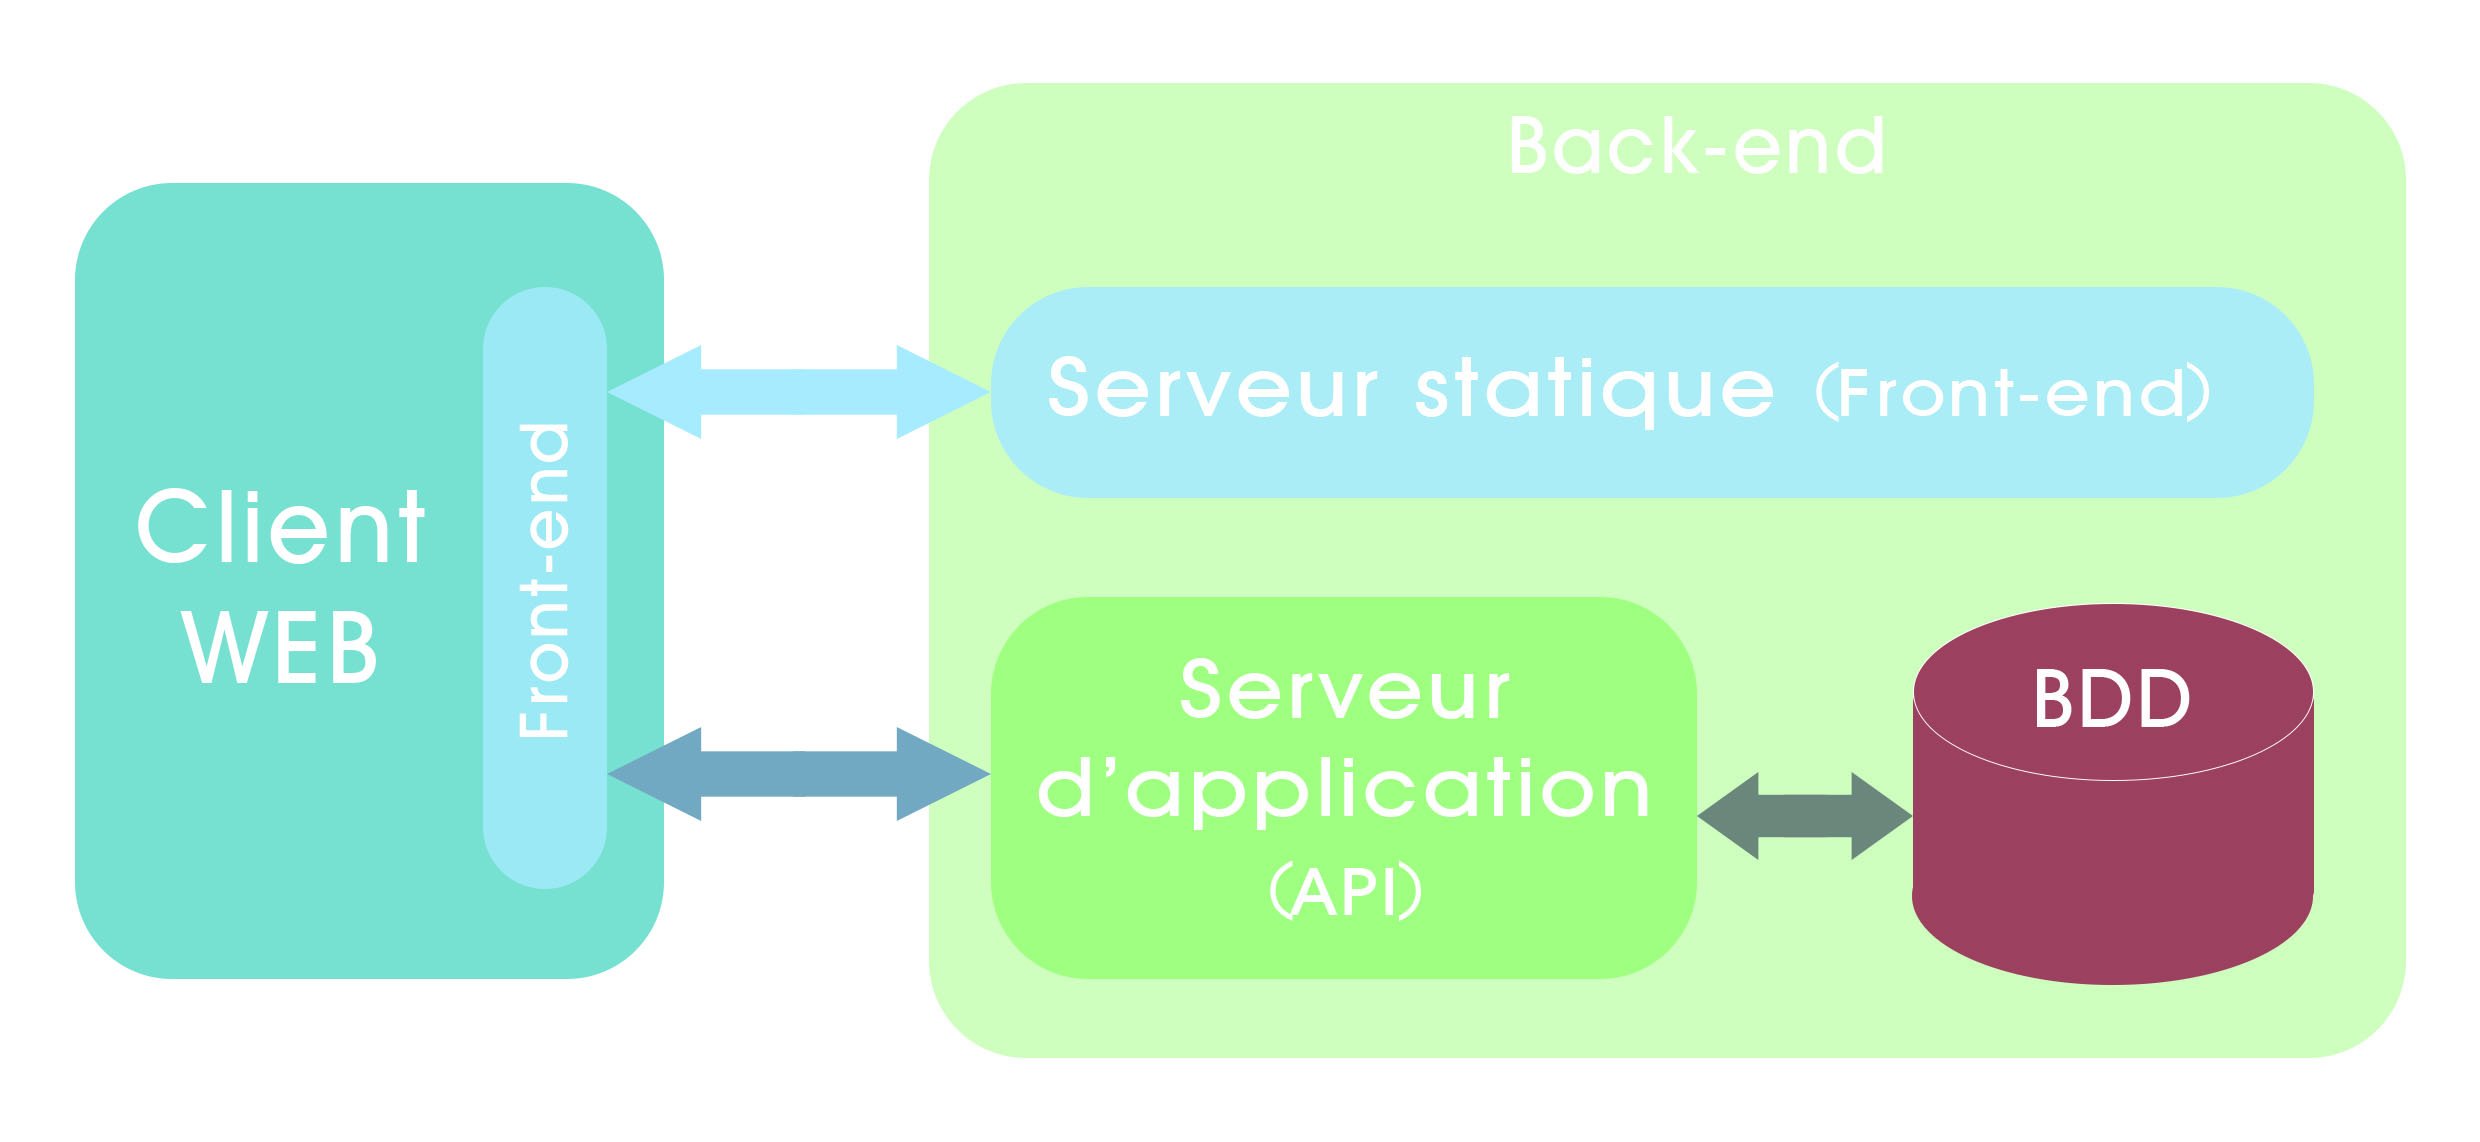
\includegraphics[width=1\linewidth]{baseArchitecture.jpg}
\caption{Architecture physique du système}
\label{fig:baseArchitecture}
\end{figure}
\

Notre système modélisé par le Back-end, chaque tiers représente l'une de ses couches. L'architecture logique du système se retrouve divisée en trois couches :
\begin{itemize}
    \item La couche d'accès aux données : Cette couche a pour charge la gestion des données du système (stockage, persistence, gestion de l'accès, ...).\\
Elle est représentée par notre base de données.
    \item La couche métier : C'est la partie fonctionnelle du système. Elle implémente la logique opératoire métier et se repose sur les données fournies par la couche inférieure. Elle offre des services à destination de la couche de présentation.\\
Elle est représentée par notre serveur d'application, qui fournit ces services sous forme d'un API.
    \item La couche de présentation : Elle encapsule l'interface utilisateur et correspond à la partie visible de l'application. Cette couche se repose sur les services offerts par la couche métier pour traiter les requêtes de l'utilisateur et s'occupe de la restitution et de la mise en forme des informations récupérées.\\
Elle est représentée par notre serveur statique, qui fournit l'application front-end au client.
\end{itemize}
\

Dans notre contexte, cette architecture en couches est la plus appropriée. L'architecture 3-tiers traditionnelle permet de bénéficier de :
\begin{itemize}
    \item Une répartition claire des responsabilités entre les couches
    \item Un couplage faible entre les différents niveaux
    \item Une simplicité lors de la réalisation de tests (la logique métier est isolée du reste des couches)
    \item Sécurité accrue, due à la séparation entre le client et les données
    \item La possibilité d'utilser des clients légers (adaptés aux dispositifs mobiles)
    \item Une évoluvité élevée, résultant de l'indépendance des couches
\end{itemize}
\

À partir de là, l'étape suivante logique pour une séparation plus aboutie des préopcupations, et donc une maintenance facilitée, a été l'orientation vers l'architecture en 4-tiers. Au travers de son adoption, nous avons clairement séparé entre l'application Front-end et l'application en charge de l'exposition de notre API. L'administration de ces deux applications sous la forme de deux projets distincts nous permet en plus de bénéficier de :
\begin{itemize}
    \item Un découplage net entre les rôles des deux applications
    \item Une évolution indépendante du Front-end
    \item Un déploiement séparé pour les deux applications
    \item Une montée en charge optimisée pour chaque entité
    \item Un versioning à part pour les deux projets
\end{itemize}
\

Les détails techniques de l'architecture seront exposés au cours des sections suivantes.

%-----------------------------------------------------------------------------------
\subsection{Technologies de base}
Pour traiter efficacement l'aspect SaaS du produit, un choix judicieux des technologies a été effectué préalablement au démarrage de la phase de développement. Nous procéderons à la présentation des technologies de base relatives à chacune des couches de notre architecture ainsi qu'à notre environnement de développement.

%-----------------------------------------------------------------------------------
\subsubsection*{Couche de présentation}
Pour réussir à développer un produit SaaS de qualité, on s'est orienté vers la mise en place d'une SPA (Single Page Application) pour la partie Front-end de notre application.\\

Dû à sa notoriété et à notre familiarité avec lui, le framework AngularJS a été notre choix de référence. L'ampleur de la communauté active développée autour de lui ainsi que l'abondance des ressources associées et le succès notoire en soi du framework nous a convaincu à l'adoption du framework en tant que brique de base pour le développement de la couche Front-end.

%-----------------------------------------------------------------------------------
\subsubsection*{Couche métier}
La couche métier de notre application nécessite le développement d'un API, dont les services seront exposés à la couche supérieure.\\
Vu les fonctionalités axées données (ressources) de notre application, nous nous sommes tournés vers la mise en place d'un API REST. En effet, dans notre cas, REST \ref{ANAGRAMME: REST} présente les avantages suivants :
\begin{itemize}
    \item L'adoption du standard HTTP en tant que protocole de communication. Son support universel assure une indépendance des technologies avec lesquelles intéragit l'API et ne restreint aucunement l'évoluvité du reste des composants.
    \item L'aspect sans état (stateless) du protocole facilite considérablement la montée en charge, considération importante à prendre en compte pour toute application en mode SaaS.
    \item Ce protocole est aussi optimisé pour l'interopérabilité avec les navigateurs (mise en cache, codes d'erreurs standards, ...) : REST représente en elle même l'architecture du web.
    \item Les Web services REST sont légers, ce qui les rend adaptés à la consommation via des dispositifs mobiles à ressources restreintes, exigence non fonctionnelle de notre application.
    \item Le support du format JSON le rend particulièrement adapté à l'interopérabilité avec le langage Javascript, qui n'est autre que le langage de dévelopement de la logique Front-end.
    \item L'abondance des technologies permettant de développer des API REST de qualité, de manière très productive.
\end{itemize}
\

Vu le succès retentissant des projets de l'entreprise d'accueil se reposant sur le langage Java, ainsi que notre familiarité avec le langage, il a été convenu dès le départ de l'adopter pour le développement en Back-end de notre produit.\\
Pour l'édification de l'API REST, nous avons favorisé l'usage de technologies conuues. C'est ainsi que nous avons opté pour l'emploi de la suite Spring. Véritable framework pour la conception de bout en bout de solutions logicielles complètes en Java, Spring offre une panoplie d'outils pour assiter à la mise en place d'un API REST. Les technologies Spring employées seront présentées en détail au cours du chapitre \ref{chap: BACKEND}.

%-----------------------------------------------------------------------------------
\subsubsection*{Couche d'accès aux données}
Pour répondre aux besoins de gestion de données de notre application, nous avons procédé à une étude approfondie des systèmes de gestion de base de données disponibles sur le marché, répondant aux critères d'exigence définis par l'entreprise d'accueil. Cette étude sera exposée durant la section \ref{section: choix SGBDR} et aboutira à la détermination de la base de données à choisir pour les besoins de la couche d'accès aux données.

%-----------------------------------------------------------------------------------
\subsubsection*{Environnement de travail}
Pour les besoins de versioning de notre travail, nous nous sommes reposés sur la solution Git.\\
Git est un logiciel libre créé par l'auteur du noyau Linux. En 2016, il s’agissait du logiciel de gestion de versions le plus populaire utilisé \ref{↑ (en) « Git 2.8.2 Popular Source Code Management System Released with Over 18 Bug Fixes » [archive] , sur Softpedia, 2 mai 2016 (consulté le 2 mai 2016)}. Il se distingue par un système de gestion de versions décentralisé.\\
Le choix de ce système de gestion de versions est judicieux dans notre cas, car il permet de garder une version complète de l'historique d'un projet en local, ce qui s'avère très utile pour le développement continue au sein et hors de l'entreprise.\\

La gestion de la liste des articles de travail ou du "Backlog" a été réalisée à l'aide de l'outil Trello.\\
Trello est à la base un outil de gestion de projet en ligne, lancé en septembre 2011, et inspiré par la méthode Kanban. Ce dernier point le rend très adapté à la gestion agile requise.

%-----------------------------------------------------------------------------------
\subsection{Choix du système de gestion de base de données}


%==============================================================================
\section*{Conclusion}
Le dénouement de la phase d'inception annonce le début de la phase de construction. Cette phase sera détaillée en long et en large au cours des prochains chapitres.

%==============================================================================
\end{spacing}
